\documentclass[Rapport/Rapport_main.tex]{subfiles}
\begin{document}
\subsection{System Arkitektur}
Indledningsvis beskrives den overordnede arkitektur for hardware og software for hele systemet. Der kan i figur \ref{fig:rap_systemarkitektur} ses et deployment view, der viser software allokeringer for de overordnede blokke.
\begin{figure}[H]
    \centering
    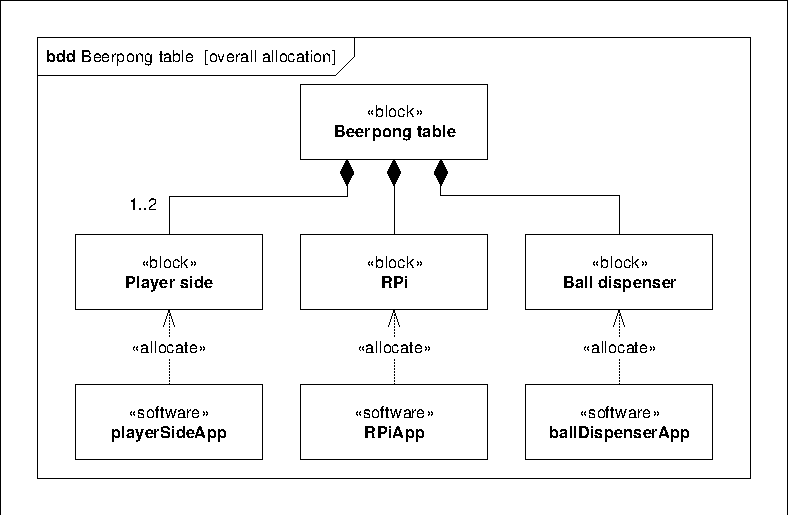
\includegraphics[width=1\textwidth,trim={0.24in 0.24in 0.24in 0.24in},clip, page=1]{Arkitektur/graphics/BDD_og_IBD.pdf}
    \caption{Overordnet blok definitionsdiagram for systemet med software allokeringer. Indeholder kun blokke der indeholder CPU. Her ses blokkene Playerside, RPi og Balldispenser. Blokkene er udledt i \textbf{Analysen} \ref{sec:rapport_analyse}}
    \label{fig:rap_systemarkitektur}
\end{figure}
Playerside blokken kan beskrives, som den blok der håndtere kopperne i enderne på bordet og som registrerer \textit{Game Events}.\\
RPi har ansvaret for kommunikationen mellem blokkene, den styre spillets gang, skriver til et display og hoster en WebServer. \\
Balldispenser står for for at håndtere indkastning af mønt, samt dispensering og overvågning af bolde.\\
De fulde blok beskrivelser kan ses i \textbf{Arktiektur} \fullref{arch:sec:system_block_description}. Efter at blokkene er defineret, så er det relevant at kigge på arkitekturen af Hardware blokkene.
\end{document}